\chapter{AsthmAPP}
\label{chp:description}

This chapter will give a description of AsthmAPP, through textual description and screenshots. Please note that the main language of the application is Norwegian. We have translated the text where it seemed appropriate. 

\section{Basic System Architecture}
\label{sec:architecture}
Figure \ref{fig:basic-architecture} shows an overview of the architecture we intend to use for our solution. We reused some of the components Aaberg et. al. created during Customer Driven Project\cite{CustomerDriven}. 

We have access to a MySQL-server hosted at NTNU, which we will access by a PHP-server hosted at NTNU. The main reason we have to access the database through a server layer, is that it is quite cumbersome to connect to the database if a device is not connected at NTNU's network. In addition, by having a webservice do some of the work for us, it becomes easier to parse results from the database through JSON. By making this choice, system scalability is reduced, but we consider this as outside the scope of our thesis.    

\begin{figure}
		\centering
			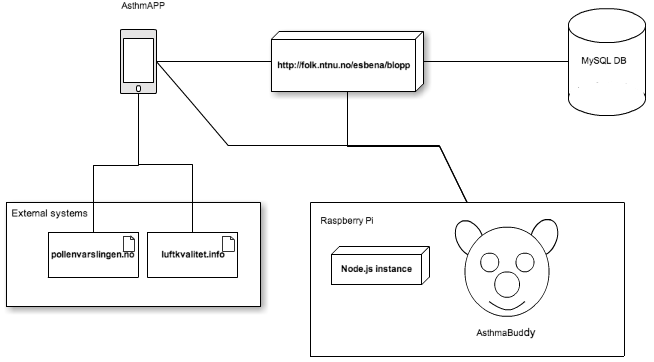
\includegraphics[width=0.60\paperwidth]{Pictures/system-architecture.png}
		\caption{System Architecture}
		\label{fig:basic-architecture}
\end{figure}

\section{How Usability Research has Affected our Design}
\label{sec:usability-affect-design}
While designing AsthmAPP, we strive for a easy-to-use design with a good overview. In chapter \ref{chp:usability} we described usability and general terms a designer should consider. We have especially taken Shneidermann's eight golden rules into consideration when designing\cite{shneiderman2003designing} in addition to the Android Design Principles\cite{androiddesign}. 
We have tried to lighten the short-term memory load by using a combination of sounds, pictures and text to tell the user what options are available or what is expected from the user. During a treatment the user is prompted to take active action in order to continue through the process, giving the user a locus of control. 
The layout for both partitions of AsthmAPP give a general overview, and has few shortcuts between the different elements. To navigate from one element to another the user will have to go via the main menu. While this breaks with Shneidermann's rules and the Android design principles, we believe that the solution we have found is the best solution.


\section{Child partition}
\label{sec:description-child-partition}
The child partition of our application consists mainly out of four parts. When Aaberg et. al. created the original application, they wanted a conceptual look and feel throughout the applications. They used images of Karotz in the application in order to introduce a sense of completeness, i.e. the Karotz bound CAPP, GAPP and KAPP together. [TODO: Vi burde bytte ut Karotz-bilder med eget produkt imo]. 

\subsection{Treatment}
\label{sec:sec:description-treatment}
Figure \ref{fig:capp_start_treatment} shows a screenshot for the application when the child starts their treatment. Starting this sequence can come from one out of two events: (i) \emph{The child reacts to an alarm set in the parent partition}, and (ii) \emph{The child needs to take their medicine by need}. If (ii) is the case, the child is instructed to pick the medicine from a list shown by the application. If (i) is the case, the medicine is chosen beforehand. When a child has started their treatment, they are taken through an animated sequence, which reacts when a child interacts with the device. In addition, they are being told what to do through the comforting voice of Andreas Ystmark.  


\subsection{Showing rewards}
\label{sec:description-show-rewards}
Figure \ref{fig:capp_stars} shows a screenshot for the application when the child wants to review how many stars he/she has received, based on the amount of treatments completed. We have made two design decisions for our reward system. First, we never want stars to be removed. We don\'t want children to feel that credits are being removed from them. Second, we can\'t assume children are able to read, and thus we have made it countable, and hopefully they can comprehend how many stars they've actually got. In addition, we provide some help to those who are able to read numbers, by showing the amount of stars a child has on the top. The downside here comes when a child has been completed a huge number of treatments, as this will obscure the view.     

\subsection{Shop}
\label{sec:description-shop}
In the shop, children are allowed to buy rewards from parents. Figure \ref{fig:child-possible-rewards} and \ref{fig:child-bought-rewards} shows an inside-view of our shop. Children can buy a reward by pressing the selected reward in the menu. Due to time constraints and lack of good software solutions, we have not been able to implement voice over, so the children might need help with reading the name of the rewards. The possibility of adding pictures to represent the reward should make it easier for children to understand. 



\subsection{Treatment instructions}
\label{sec:description-instructions}
The treatment instructions is a book-styled instruction set which shows generically how to take a medicine. 
The following steps are included in instructions: 
\begin{enumerate}
  \item Shake the inhaler to loosen the particles. 
  \item Take the cap of the inhaler
  \item Attach the inhaler to the inhaling chamber
  \item Cover nose and mouth with the inhaling chamber
  \item Press the inhaler until you hear a sound
  \item Let the child breathe calmly 10 times in and out
  \item Let the child wash his/her mouth
\end{enumerate} 

\begin{figure}
	\begin{minipage}[t]{0.25\linewidth}
		\centering
			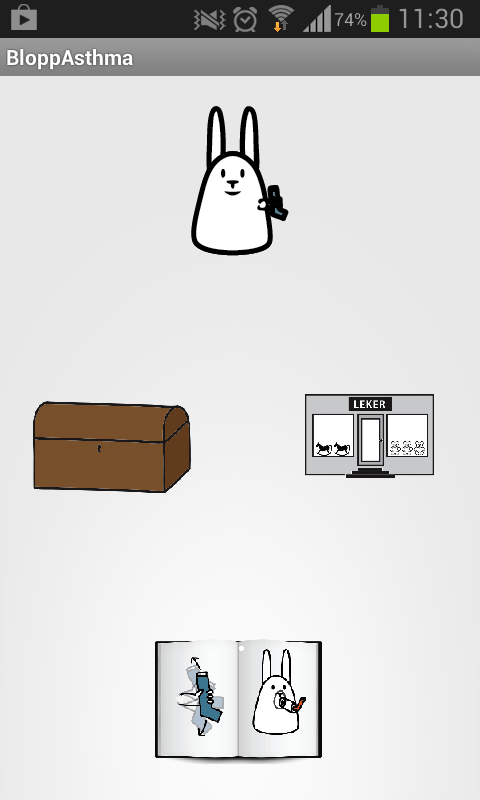
\includegraphics[width=0.20\paperwidth]{Pictures/new-screenshots/kid-menu.png}
		\caption{Main menu of child partition}
		\label{fig:child-menu}
	\end{minipage}
	\hspace{1cm}
	\begin{minipage}[t]{0.25\linewidth}
		\centering
			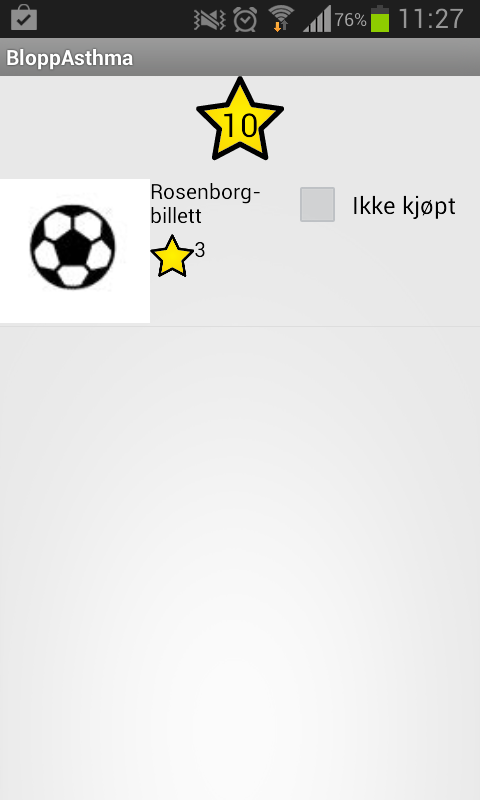
\includegraphics[width=0.20\paperwidth]{Pictures/new-screenshots/child-possible-rewards.png}
		\caption{Possible rewards a child can choose from}
		\label{fig:child-possible-rewards}
	\end{minipage}
	\hspace{1cm}
	\begin{minipage}[t]{0.25\linewidth}
		\centering
			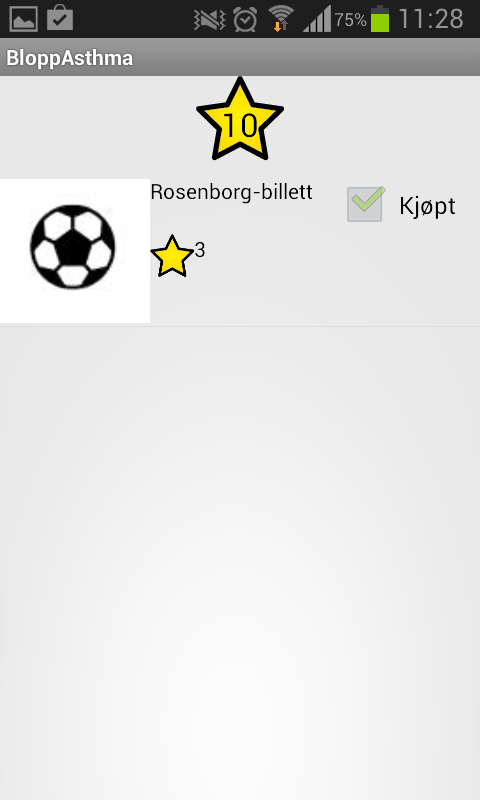
\includegraphics[width=0.20\paperwidth]{Pictures/new-screenshots/child-bought-reward.png}
		\caption{A child has bought the reward}
		\label{fig:child-bought-rewards}
	\end{minipage}
\end{figure}

\begin{figure}
	\begin{minipage}[t]{0.4\linewidth}
		\centering
			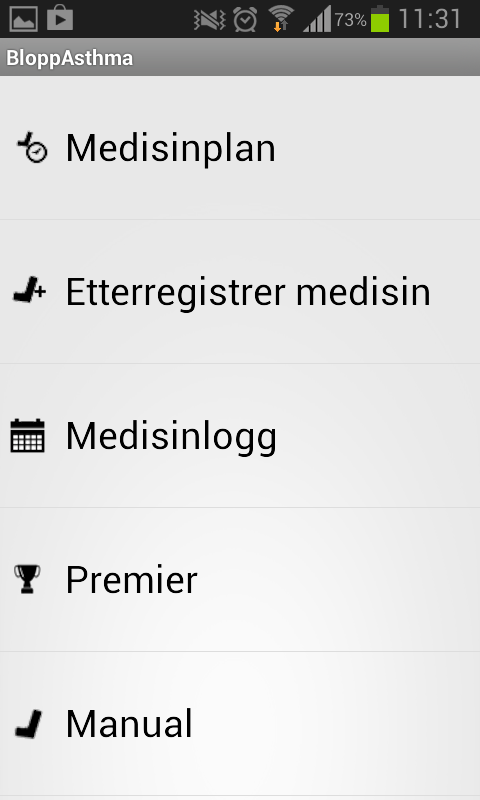
\includegraphics[width=0.20\paperwidth]{Pictures/new-screenshots/parent-menu.png}
		\caption{Main menu of partent partition}
		\label{fig:parent_main_menu}
	\end{minipage}
	\hspace{3cm}
	\begin{minipage}[t]{0.4\linewidth}
		\centering
			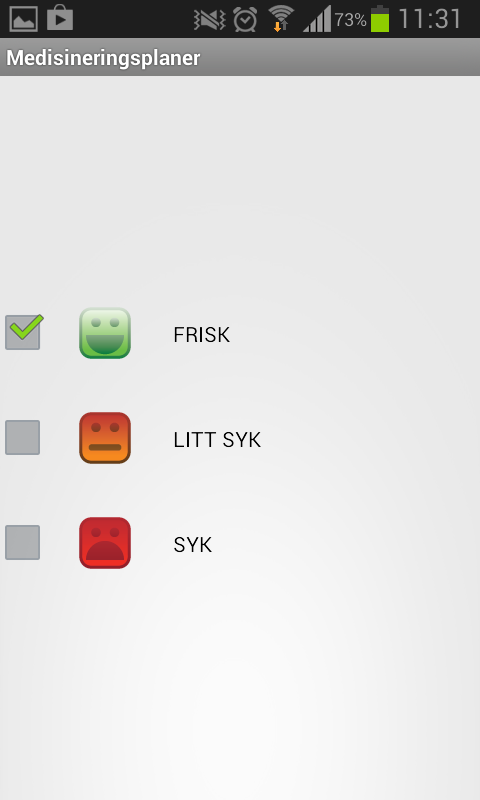
\includegraphics[width=0.20\paperwidth]{Pictures/new-screenshots/medicine-plans.png}
		\caption{Available medicine plans}
		\label{fig:parent_medicine_plans}
	\end{minipage}
	%NEW LINE
	\begin{minipage}[t]{0.4\linewidth}
		\centering
			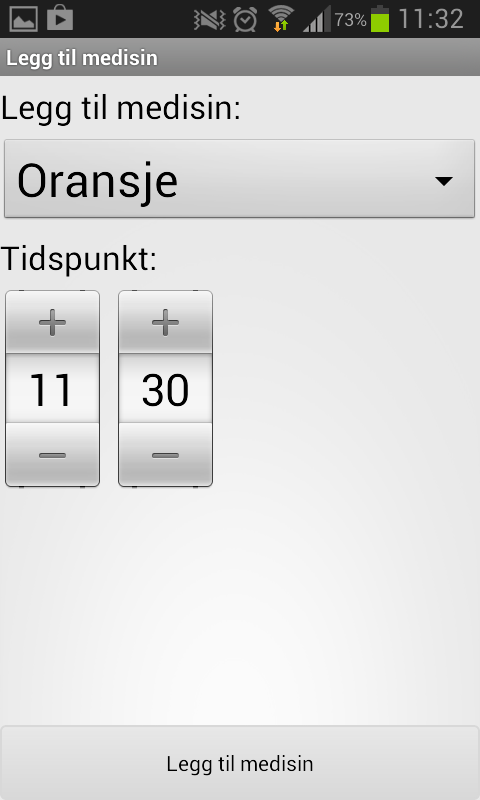
\includegraphics[width=0.20\paperwidth]{Pictures/new-screenshots/add-medicine-to-plan.png}
		\caption{Adding a medicine to a plan}
		\label{fig:add_medicine_to_plan}
	\end{minipage}
	\hspace{3cm}
		\begin{minipage}[t]{0.4\linewidth}
		\centering
			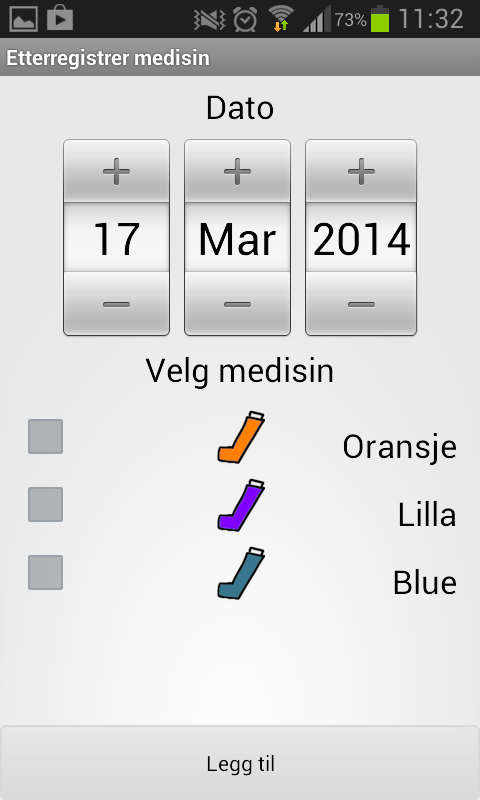
\includegraphics[width=0.20\paperwidth]{Pictures/new-screenshots/register-medicine-taken.png}
		\caption{Register a medicine that was taken without the help of \buddy{} or AsthmAPP}
		\label{fig:register_medicine_taken}
	\end{minipage}
	%NEW LINE
		\begin{minipage}[t]{0.4\linewidth}
		\centering
			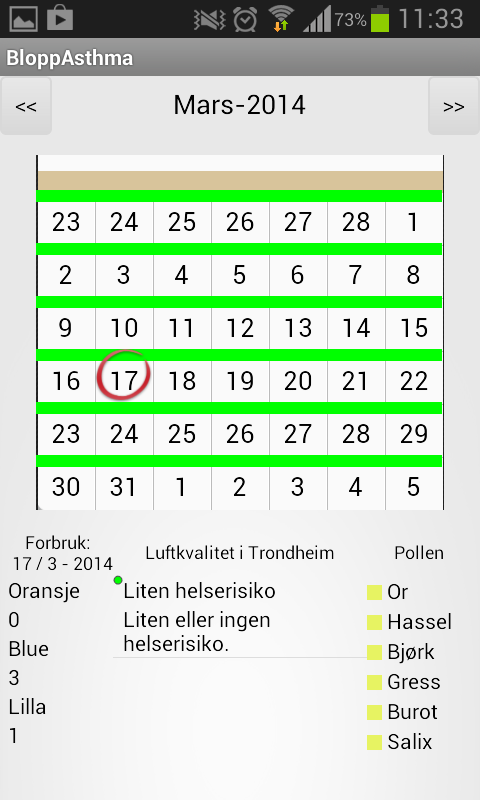
\includegraphics[width=0.20\paperwidth]{Pictures/new-screenshots/log.png}
		\caption{Medicine log}
		\label{fig:medicine-log}
	\end{minipage}
	\hspace{3cm}
		\begin{minipage}[t]{0.4\linewidth}
		\centering
			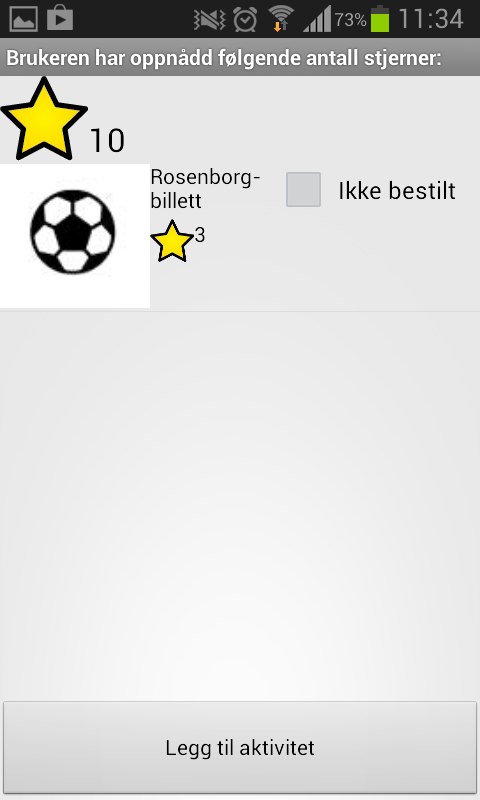
\includegraphics[width=0.20\paperwidth]{Pictures/new-screenshots/award.png}
		\caption{Overview of rewards a child can get}
		\label{fig:parent-awards}
	\end{minipage}
\end{figure}

\begin{figure}
	\begin{minipage}[t]{0.4\linewidth}
		\centering
			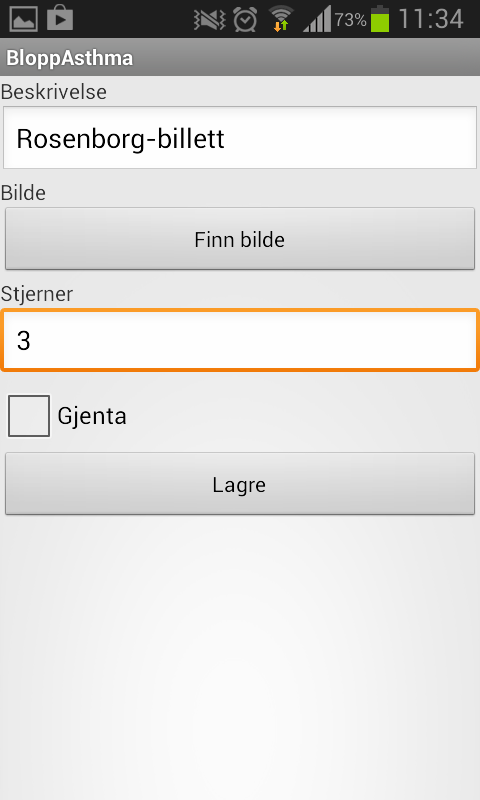
\includegraphics[width=0.20\paperwidth]{Pictures/new-screenshots/create-award.png}
		\caption{Creating a reward. Parents can either choose a reward from our standard image set, or they can take one from their gallery}
		\label{fig:parent-create-reward}
	\end{minipage}
	 \hspace{3cm}
	 \begin{minipage}[t]{0.4\linewidth}
		\centering
			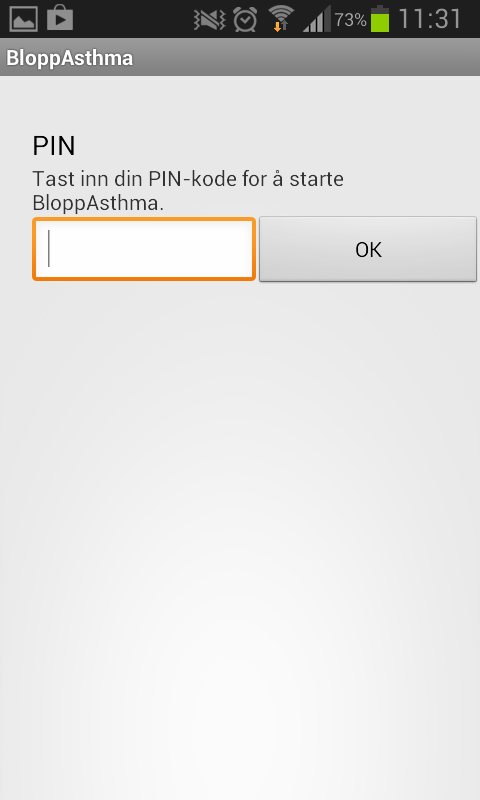
\includegraphics[width=0.20\paperwidth]{Pictures/new-screenshots/pin-challenge.png}
		\caption{In order to access the parent partition, users have to complete a PIN-challenge}
		\label{fig:parent-pin}
	\end{minipage}
\end{figure}

\section{Parent Partition}

\subsection{Menu}
\label{sec:description-menu}
Figure \ref{fig:parent_main_menu} shows the main menu of the parent partition. It has six options (Norwegian translation in paranthesis):
\begin{enumerate}
  \item Medicine Plan (\emph{Medisinplan})
  \item Register Medicine Afterwards (\emph{Etterregistrer medisin})
  \item Medicine Log (\emph{Medisinlogg})
  \item Rewards (\emph{Premier})
  \item Manual (\emph{Manual})
\end{enumerate} 

In order to access the parent partition, the user is prompted with a PIN challenge. This was an effort to anonymize children's medical data if a phone is lost or stolen. 

\subsection{Medicine plan}
\label{sec:description-medicine-plan}
Creating a medicine plan for asthma treatment is highly connected to the Traffic Light System explained in Appendix \ref{chp:traffic-light}.
Users can have three different plans, depending on which health state they are currently in. As we are targeting children, we can not assume that they are aware of which category they are currently in, and as a result, we let their parents control it. Figure \ref{fig:gapp-view-plans} and \ref{fig:add_medicine_to_plan} shows the view in which one may the change medicine plan their child are currently on, in addition to setting alarms where appropriate. For instance, one might set an alarm at 07:00, which makes the user aware before it is time to leave for school. Changing medicine plan is done by selecting the checkbox at the left side of the panel.  


\subsection{Register Treatment}
\label{sec:description-register-medicine}
What happens if a child need their medicine, but the application or our TUI is not nearby? They would probably be disappointed because they did not get their star, and did not get any rewards. Fortunately, it is possible to register a medicine that has been taken afterwards, which entitle the child the amount of stars they should have gotten. \emph{Register Treatment} allows parents to register the medicine, at any given day prior to current time (See Figure \ref{fig:register_medicine_taken}).  


\subsection{Medicine log}
\label{sec:description-medicine-log}
The \emph{Medicine log} can be used by parents to show how many times a child has taken their medicine. One of the main reasons that children does not take their medicine is lack of communication between parents. Having an option to show medicine log, give parents the ability to check and see whether they have taken the necessary amount at a given day.

Figure \ref{fig:medicine-log} shows the calendar view of the application. The view is a bit complicated. The cells show any given day of a month. In addition, there is a top bar in the view. The top bar indicates which health state (or health plan) the child was in at the day represented below. At the bottom of the screen, there are three panels. The left one shows which medicine that has been taken at a selected day. The topbar indicates which day is shown. The middle one shows the air quality in Trondheim \fnurl{Measured by NILU}{http://luftkvalitet.info/}. The right shows the pollen distribution of the 6 most common pollen types \fnurl{Measured by NAAF}{http://www.pollenvarslingen.no/}. The idea behind this is that asthma symptoms can often be the same as allergy symptoms, and if parents are able to recongize a pattern between health state and pollen distribution, they might want to take their child to a hospital.    


\subsection{Manual}
\label{sec:description-manual}
The manual contains excactly the same information as shown in Section \ref{sec:description-instructions}. The manual is added to both the parent partition and the child partition of the application. This is done because it is important for both the children and the parents to know how to use the medicine correctly. 


\subsection{Reward}
\label{sec:description-manage-rewards}
Figure \ref{fig:parent-awards} shows the list of possible rewards a child might receive. They are added by parents through \emph{Add reward}. The idea of having parents set their children's rewards is to specify rewards according to children's interest (see Section \ref{sec:gamificationinapp}). Figure \ref{fig:parent-create-reward} shows how one may add a reward. Users inserts a description, then either take a photo or select one out of our standard images. It is possible to set a reward on \emph{Repeat}, which will make the reward appear multiple times, each time with an increased cost.        
When the user press \emph{Save} (Lagre), the reward is added and children have the possibility to buy it. 
 
 
\section{Evaluation}

Chapter \ref{chp:gamification} gave an introduction to the term gamification, and how it should be used. We have developed a reward system that is highly based on parent's opinions, and thus, have some flaws that we'll discuss further here.

First of all, children might become bored of the rewards if the rewards are not increased in difficulty to achieve, and their apparent value. For instance, if a child is rewarded with a ticket to a football match for achieving 10 stars, and then gets a piece of gum if they achieve 20 stars, they will easily lose interest and important motivation in order to do their treatment. 

Second, the amount of stars is rewarded depending upon their inferred health state (green state yields 1 star, orange state yields 3 stars and red state yields 5). This could be easy for a ``sneaky'' child to social engineer. In the long run, a child could fake being sicker than he or she actually is, just in order to achieve a reward more easily. This is a grayzone flaw that \emph{could} occur, but we did not have the possibility to observe this pattern over time.

Third, the gamification during their treatment, i.e. the animation on the phone, could become boring over time. 
The interactions are not variated, and it takes approximately [X] minutes to go through with a treatment. For expert users, who have had asthma for several years, it will become boring. Thus it should be noted that this is an application that probably would work best for children in the early stage of their disease.      

In order to get some expert opinion on our reward system, we asked a child psychologist with expertise about our system. 

[Include comments here] 


